\subsection{Evaluation of \name}
\label{minjia_subsec:eval-hmann}

\textbf{Billion-scale algorithm comparison.} We compare \algoname with the graph- (HNSW and NSG) and quantization-based algorithms (IMI+OPQ and L\&C).
For HNSW, we build graphs with $efConstruction$ and $M$ set to 200 and 48 respectively; For NSG we first build a 100-NN graph using Faiss~\cite{faiss} and then build NSG graphs with R = 128, L = 70 and C = 500. 
We collect results on NSG and HNSW using Memory Mode since it leads to overall better performance than using first-touch NUMA.
For IMI+OPQ, we build indexes with 64- and 80-byte code books on BIGANN and DEEP1B respectively. We present the best search result with search parameters nprobe=128 and ht=30 for BIGANN and with autotuning parameter sweep on DEEP1B. For L\&C,  we use 6 as the number of links on the base level, and use 36- and 144-byte OPQ code-books. We use the same parameters ($efConstruction$=200 and $M$=48) as HNSW to construct \name. We set $efSearch_{L0}$=2 and vary $efSearch_{L1}$ to show the latency-vs-recall trade-offs.

Figures~\ref{minjia_fig:billion} (a)-(d) visualize the results. Overall, \algoname provides the best latency-vs-recall performance. Figure~\ref{minjia_fig:billion} (a) and (b) show that \algoname achieves the top-1 recall of $>95\%$ within 1ms, which is 2x and 5.8x faster than HNSW and NSG to achieve the same recall target respectively.  
IMI+OPQ and L\&C cannot reach a similar recall target, because of precision loss from quantization. As another point of reference, the SSD-based solution, DiskANN~\cite{diskann} (not open-sourced), provides 95\% top-1 recall in 3.5ms. In contrast, \name provides the same recall in less than 1ms, which is at least 3.5\(\times\) faster.
We compare the top-100 recall shown in Figures~\ref{minjia_fig:billion} (c) and (d). \algoname provides higher performance than all other approaches. For example, it obtains top-100 recall of $>90\%$ within 4 ms, while performing 2.8x and 5x faster than HNSW and NSG with the same recall target respectively. Quantization-based algorithms perform poorly and have difficulties to reach a top-100 recall of 30\%. 

\begin{table}
\newcommand{\colspc}{\hspace*{0.4em}}
\caption{Indexing time and memory consumption for graph-based methods on billion-scale datasets}\label{minjia_tab:indexing_time_and_mem_for_1b}
\centering
\scriptsize
\begin{tabular}{|@{\colspc}c@{\colspc}|@{\colspc}c@{\colspc}|@{\colspc}c@{\colspc}|@{\colspc}c@{\colspc}|@{\colspc}c@{\colspc}|@{\colspc}c@{\colspc}|@{\colspc}c@{\colspc}|@{\colspc}c@{\colspc}|@{\colspc}c@{\colspc}|@{\colspc}c@{\colspc}|@{\colspc}c@{\colspc}|}
\hline
\multirow{3}{*}{}                   & \multicolumn{5}{c|}{\textbf{BigANN}}  & \multicolumn{5}{c|}{\textbf{DEEP1B}}               \\ \cline{2-11} & \multicolumn{3}{c|}{\textbf{Indexing}}      & \multicolumn{2}{c|}{\textbf{Search}}                      & \multicolumn{3}{c|}{\textbf{Indexing}}                    & \multicolumn{2}{c|}{\textbf{Search}}                    \\ \cline{2-11} & \centering \begin{tabular}[c]{@{}c@{}}Graph\\  size\end{tabular} &\centering \begin{tabular}[c]{@{}c@{}}Indexing\\  time\end{tabular} & \begin{tabular}[c]{@{}c@{}}Promo.\\  rate\end{tabular} & \centering \begin{tabular}[c]{@{}c@{}}Fast-mem \\ usage\end{tabular} & \begin{tabular}[c]{@{}c@{}}Slow-mem\\  usage\end{tabular} & \begin{tabular}[c]{@{}c@{}}Graph\\  size\end{tabular} & \begin{tabular}[c]{@{}c@{}}Indexing\\  time\end{tabular} & \begin{tabular}[c]{@{}c@{}}Promo.\\  rate\end{tabular} & \centering \begin{tabular}[c]{@{}c@{}}Fast-mem \\ usage\end{tabular} & \begin{tabular}[c]{@{}c@{}}Slow-mem\\ usage\end{tabular} \\ \hline
\multicolumn{1}{|c|}{\textbf{HNSW}} & 475GB  &\centering 90h    &\centering 0.02    & \begin{tabular}[c]{@{}c@{}}96GB\\  (hw caching)\end{tabular}  &\centering 490GB  &\centering 723GB   & \centering 108h &\centering 0.02  & \begin{tabular}[c]{@{}c@{}}96GB\\  (hw caching)\end{tabular} &\centering 748GB  \tabularnewline \hline
\multicolumn{1}{|c|}{\textbf{NSG}}  & 285GB   &\centering 115h &\centering -   & \begin{tabular}[c]{@{}c@{}}96GB\\  (hw caching)\end{tabular} &\centering 303GB  & 580GB  &\centering 134h &\centering -   & \begin{tabular}[c]{@{}c@{}}96GB\\  (hw caching)\end{tabular}  &\centering 599GB   \tabularnewline \hline
\multicolumn{1}{|c|}{\textbf{\name}} & 536GB    &\centering 96h  &\centering 0.16  & \centering 96GB &\centering 462GB  & 756GB  &\centering 117h  &\centering 0.11 &\centering 96GB   &\centering 681GB               \tabularnewline \hline
\end{tabular}
\end{table}

Table~\ref{minjia_tab:indexing_time_and_mem_for_1b} shows the index construction time and index size of HNSW, NSG, and \name. Among the three, HNSW takes the shortest time to build the graph. \name takes 8\% longer time than HNSW because it takes an additional pass for the bottom-up promotion. However, \name is still faster to construct than NSG.
In terms of memory usage, \name indexes are 5--13\% larger than HSNW, because it promotes more nodes from L0 to L1. %(i.e., higher promotion rates).
In terms of memory usage, \name consumes less fast memory than HNSW and NSG, which is valuable to reduce production cost~\cite{ram_price,ram_price2}.
HNSW and NSG use all fast memory because they do not explicitly manage HM and by default using Memory Mode consumes all fast memory. The sum of slow and fast memory consumption can be larger than the index size because there are metadata needed for search that are not counted in the index size.

\begin{figure*}[!ht]
 \centering
 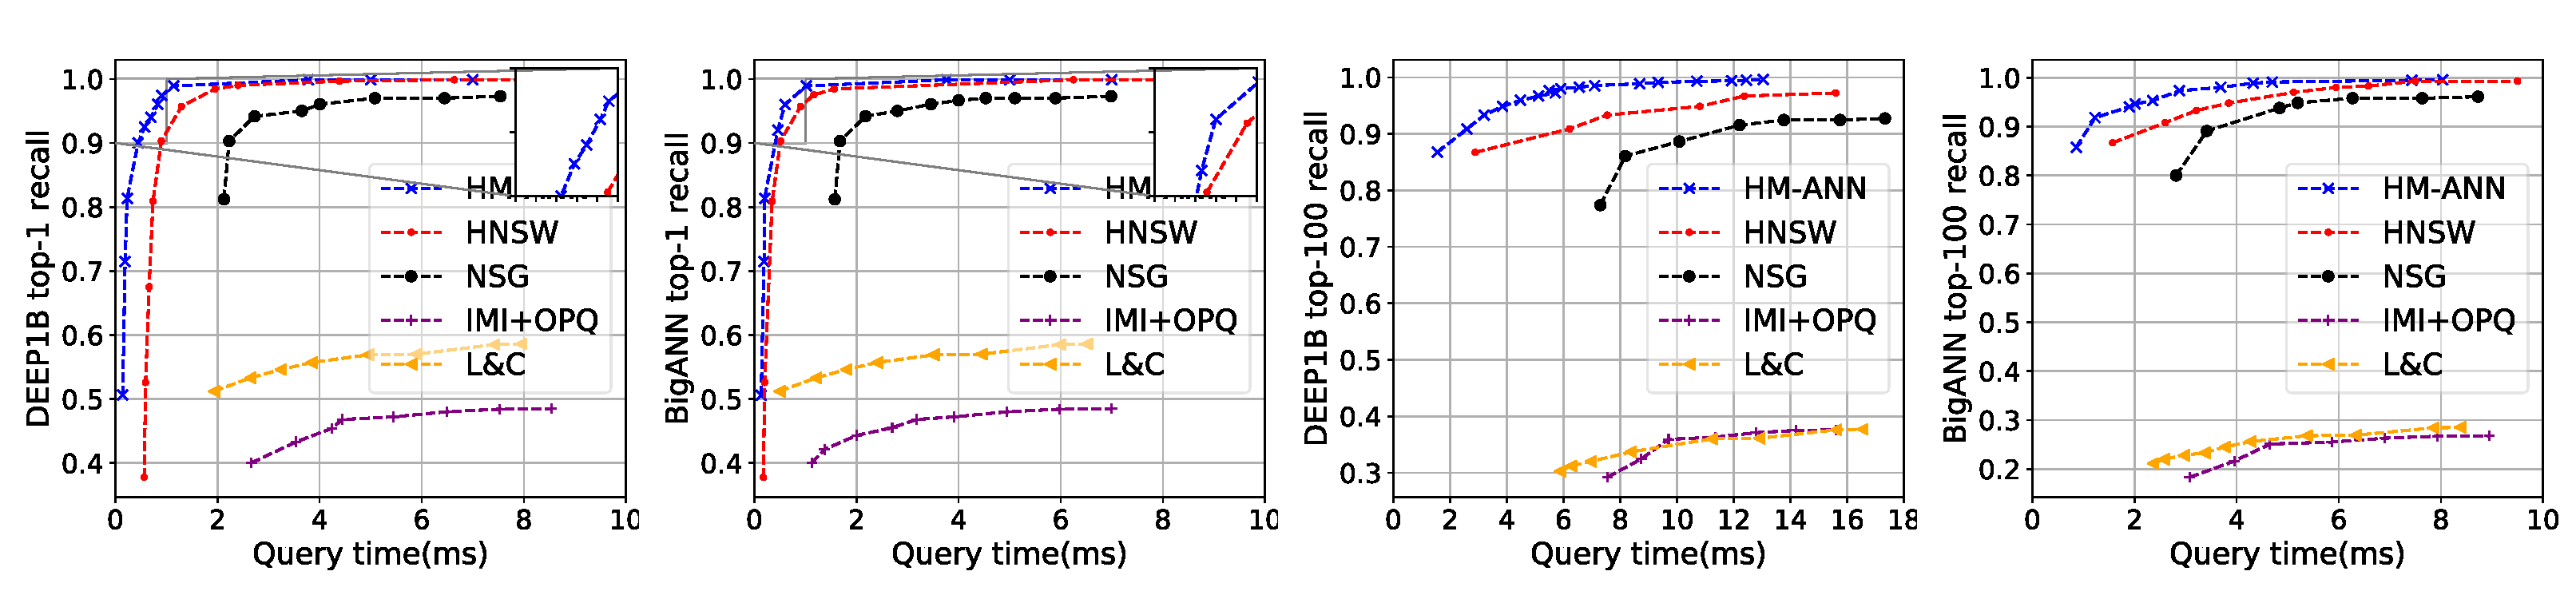
\includegraphics[width=\linewidth]{submissions/Minjia2023/figures/billion_result.pdf}
 \caption{Query time vs. recall curve in (a) DEEP1B top-1, (b) BigANN top-1, (c) DEEP1B top-100, (b) BigANN top-100, respectively.}\label{minjia_fig:billion}
\end{figure*}